
\section{Loss Function Development Story}


Our proposed \geom{} loss function can be rewritten as shown in \cref{eq:objective}.
\begin{equation}\label{eq:objective}
\begin{split}
    \mathcal{L}  &= \sum_{i=1}^{M-1} \sum_{j=i+1}^{M} dist( z_{i}^{+} , z_{j}^{+}) 
     - dist( z_{i}^{+} , z_{j}^{-}) - dist( z_{i}^{-} , z_{j}^{+}) - \sum_{i=1}^{M} dist( z_{i}^{+} , z_{i}^{-} )
\end{split}
\end{equation}


We designed and experimented with alternative versions of our \geom{} loss function to analyze if they offer better results.
We start with a modification of the triplet loss function idea where we fix one modality as anchor and do not sample a positive instance from the same modality. 
Na\"ively, to extend triplet loss to work with arbitrary number of modalities, we can use two anchors (e.g., text and speech), which results in $2(M-2)$ triplet losses as formulated in~\cref{eq:objective-two-anchors}. 

% \todoffinline{in this equation block, you're writing things like $|| z_{t}^{+} - z_{m}^{+} ||$. Do you actually mean norm, or would any old scoring function work?}

\begin{equation}
\label{eq:objective-two-anchors}
\begin{split}
    \mathcal{L}  &= \sum_{m=1}^{M-2} dist( z_{t}^{+} , z_{m}^{+} ) - dist( z_{t}^{+} , z_{m}^{-} ) + dist( z_{s}^{+} , z_{m}^{+} ) - dist( z_{s}^{+} , z_{m}^{-} ) \\
    &= \sum_{m=1}^{M-2} \cos(z_{t}^{+} ,z_{m}^{-}) - \cos(z_{t}^{+}, z_{m}^{+}) + \cos(z_{s}^{+} ,z_{m}^{-}) - \cos(z_{s}^{+}, z_{m}^{+})
\end{split}
\end{equation}
where $M$ is the number of modalities, $t$ represents text modality, $s$ represents speech modality, and the superscripts $+$ and $-$ represent positive and negative objects, respectively.
The $\cos(\cdot)$ function is a measure of similarity, not distance, and that is why the signs are reversed. To measure the distance, we use cosine distance.
In order to use cosine \textit{distance}, we have to subtract the cosine of the \textit{angle} between two embeddings (which represents similarity) from 1: $1 - \cos(e_1, e_2)$.

However, this approach performs poorly when one of the anchor modalities is ablated; since there is no explicit minimization between the two anchors, text (t) and speech (s) do not necessarily map closely to each other, such that only one of the two anchors is actually learned. 





An alternative is to apply triplet loss $M-1$ times with a single fixed anchor (text in our case) and $M-1$ `target' modalities.  In this case, the negative anchor point is disregarded. The positive anchor is used as an anchor for all $M-1$ triplet losses, and for each of those triplet losses the positive and negative points are simply selected from the corresponding modalities. This can be derived from \cref{eq:full-emma} by fixing one modality as anchor, and excluding the distance between the positive and negative anchors or $\cos(z_{a}^{+}, z_{a}^{-})$.
\Cref{eq:objective-simple-mma} formulates this idea.

\begin{equation}
\label{eq:objective-simple-mma}
\begin{split}
    \mathcal{L}  &= \sum_{m=1}^{M-1} dist( z_{a}^{+} , z_{m}^{+} ) - dist( z_{a}^{+} , z_{m}^{-} ) \\
    &= \sum_{m=1}^{M-1} 1 - \cos(z_{a}^{+}, z_{m}^{+}) - (1 - \cos(z_{a}^{+}, z_{m}^{-})) \\
    &= \sum_{m=1}^{M-1} \cos(z_{a}^{+} ,z_{m}^{-}) - \cos(z_{a}^{+}, z_{m}^{+})
\end{split}
\end{equation}
Here, subscript $a$ represents the \textit{anchor} modality, $M$ is the number of modalities, superscript $+$ represents the positive objects, and superscript $-$ represents the negative objects.

However, this approach fails to take into account the dissimilarity of the positive and negative anchor points. This is an important piece of information that \cref{eq:objective-simple-mma} ignores. Although this information is implicitly captured when we maximize the distance between positive anchor and other negative modalities, when the negative data point becomes a positive example itself, the anchor and those points are forced to be closer to each other which can happen in three ways: either moving anchor closer to those points, moving those points closer to anchor, or move both somewhere in between. Therefore, in the last two cases we do not have explicit direct control over the distance between these points and previous positive points. Our experimental results confirm this hypothesis.

Therefore, we add an extra term which is responsible for maximizing the distance between positive and negative instances of the anchor modality, because a margin between positive and negative points from other modalities (excluding anchor) is enforced. This can be derived from \cref{eq:full-emma} by fixing one modality as anchor.
% The first dashed line from the top in \cref{fig:emma-loss} is this extra term that captures the dissimilarity between positive and negative text datapoints.
We formulate this method in \cref{eq:objective-explicit-fixed-anchor}, which is generalized to an arbitrary number of modalities.

\begin{equation}
\label{eq:objective-explicit-fixed-anchor}
\begin{split}
    \mathcal{L}  %&= %\sum_{m=1}^{M-1} || z_{a}^{+} - z_{m}^{+} || - || z_{a}^{+} - z_{m}^{-} ||  - || z_{a}^{+} - z_{a}^{-} || \\
    &= \max(\cos(z_{a}^{+}, z_{a}^{-}) + \alpha_a, 0) + \sum_{m=1}^{M-1} \max \left(\cos(z_{a}^{+} ,z_{m}^{-}) - \cos(z_{a}^{+}, z_{m}^{+}) + \alpha_m, 0 \right) \\  
    &= \sum_{m=1}^{M}  \cos(z_{a}^{+} ,z_{m}^{-}) - \sum_{m=1}^{M-1} \cos(z_{a}^{+}, z_{m}^{+})
\end{split}
\end{equation}


In \cref{eq:objective-explicit-fixed-anchor}, $a$ represents the \textit{anchor} modality, $M$ is the number of modalities, the superscripts $+$ and $-$ represent positive and negative objects, $\alpha_m$ represents enforced margin for each modality which we set to 0.4 for all modalities without tuning, and $z$ is the embedding we get by applying a mapping function $f$, which in our case is a neural network on our input data.
In other words, $z_m = f_m(x_m)$, where each modality $m$ has a specific model $f_m$ that is different from the models for other modalities. These models do not share their weights.

Since the downstream task we are considering in the grounded language learning domain is to predict/retrieve a desired object among multiple objects given a natural language description, it makes sense to train the model using language as an anchor, and in fact anchoring learning around language outperforms anchoring on RGB. However, our proposed \geom{} loss function formulated in \cref{eq:full-emma} where we treat all modalities as anchor once still results in a better performance.


% Triplet loss cannot be used for more than 2 modalities. Some previous work has concatenated RGB and depth embeddings to create a single ``vision'' embedding for learning~\cite{triplet_loss_2021_CVPR}, but they cannot handle RGB or depth sensor ablation during test. Since our method can handle any number of modalities, we can handle such a case by treating depth as a separate modality.
% Moreover, when using triplet loss with different anchors per batch, the batch size has to be 1 which makes training very slow.

% This approach is most similar to that of supervised contrastive learning~\cite{NEURIPS2020_supervised_contrastive}, but outperforms both that and regular contrastive learning~\cite{chen2020simple} methods.
% Especially when modalities are ablated, most notably written language.

% We find that the use of instance level losses grounded to one key modality (text) is sufficient to encourage a representation that satisfies our goals. 






\subsection{Extended Triplet}
Using an extended version of triplet loss to consider all pairwise connections which is formulated in \cref{eq:extended-triplet}, results in a worse performance.

\begin{equation}\label{eq:extended-triplet}
    L = \sum_{m_1=1}^{M} \left[ \sum_{m_2=m_1+1}^{M} \left[ \text{triplet}(z_{m_1}^{+}, z_{m_2}^{+}, z_{m_2}^{-}) + \text{triplet}(z_{m_1}^{-}, z_{m_2}^{-}, z_{m_2}^{+}) \right] + \cos(z_{m_1}^{+}, z_{m_1}^{-}) -1 + margin \right]
\end{equation}

% Didn't change much when we drop text: Full eMMA when we have similar objects 

% Did not work: Run the version with all connections (including among negatives) without triplet and just by using cosine distance between pair of embeddings



\subsection{Smaller Batch Sizes And Pulling Among Negatives}

Reducing the batch size from 64 to 16 and 8 (for both \ours{} and \supcon{}) increases the gap between our model and the baseline in cases where our model beats the baseline (all modalities, dropping speech), but baseline is still better than ours when we drop the text modality.

In batch size of 2 the trend is still the same, but when we drop the text modality, the MRR graph is flat at 0.4. This is still better than the worst and random cases, but it implies that the model does not learn anything with regards to speech.
To remedy this, we add connections among the modalities of the negative instance as formulated in \cref{eq:full-emma-pull-negatives} and as shown in \cref{fig:full-emma-pull-negatives}, and that solves the flatline problem when we drop the text modality; however, when we have all modalities it performs worse than \ours{}.

\begin{equation}\label{eq:full-emma-pull-negatives}
\begin{split}
    L = & \sum_{m_1=1}^{M} \left[ \sum_{m_2=1}^{M} \left[ \max (\cos(z_{m_1}^{+}, z_{m_2}^{-}) -1 + margin,0) \right] + \sum_{m_3=m_1+1}^{M} \left[ \max(1 - \cos(z_{m_1}^{+},z_{m_3}^{+}),0) \right] \right. \\
    & \left. + \sum_{m_3=m_1+1}^{M} \left[ \max(1 - \cos(z_{m_1}^{-},z_{m_3}^{-}),0) \right] \right]
\end{split}
\end{equation}

\begin{figure*}[tb]
\centering
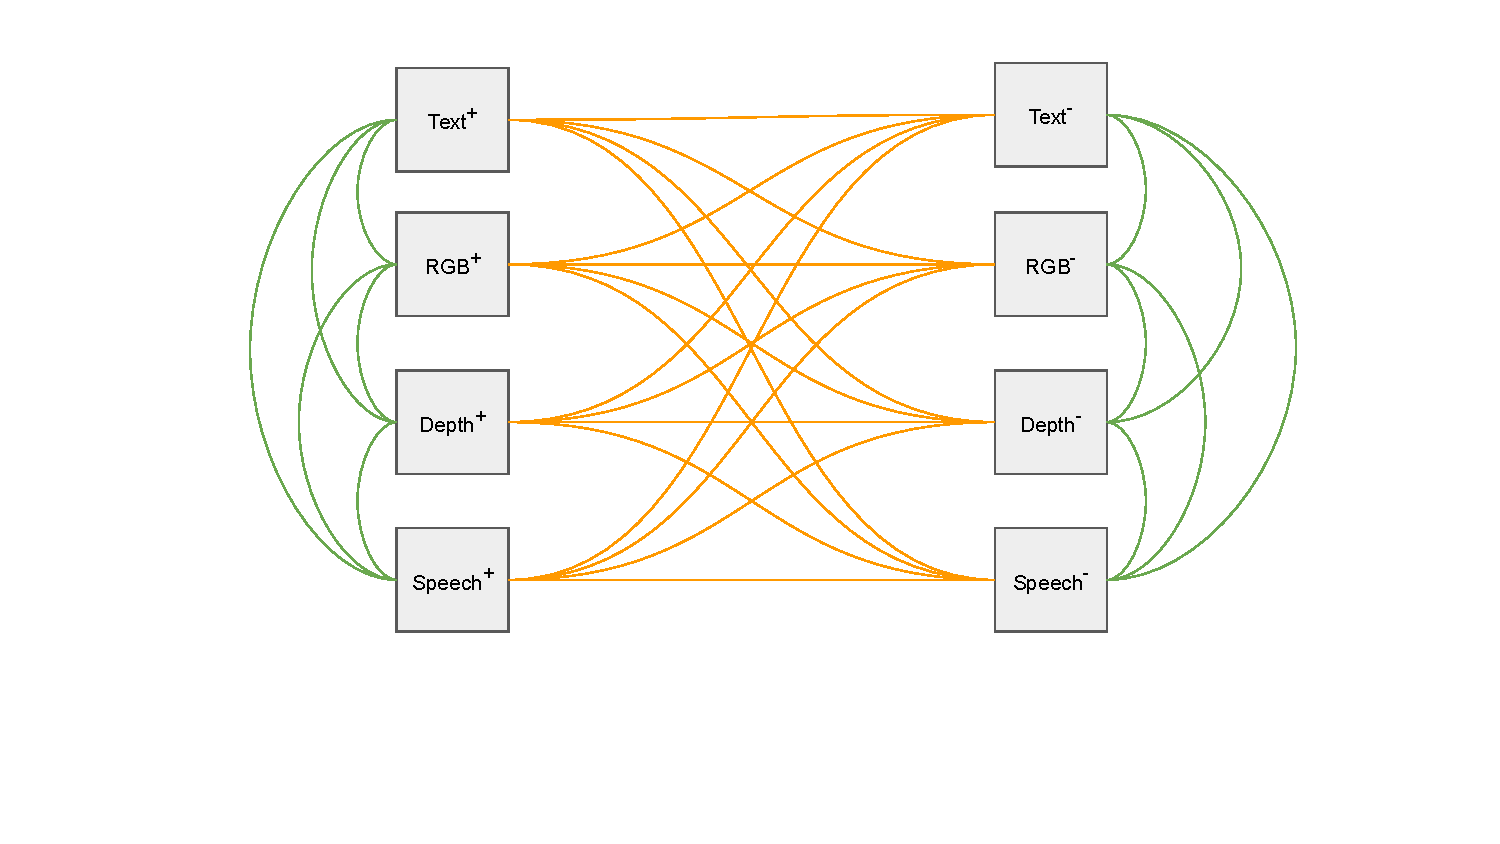
\includegraphics[width=1\columnwidth]{Figures/unused/full-emma-pull-negatives.pdf}
\caption{A high-level prototype of our approach and the distances used when we have add pulling among negative modalities.}
\label{fig:full-emma-pull-negatives}
\end{figure*}



\subsection{Margin}
% \todokdinline{Try different margins of 0.6, 1.0, and if it improved the results we can try to learn it as a parameter}
% \todokdinline{Should we remove this section?}
We experimented with two different margins values: a margin of 0.6 and a margin of 1.0. Using a margin of 0.6 does not change the performance much. However, it converges even faster. Using a margin of 1.0 (this is essentially just cosine similarity because we have $cos -1 + \text{margin}$) results in a worse performance when we have all modalities. 
% The MRR is 0.8995 when margin is 1, while with a margin of 0.6 the MRR is 0.9176, and with a margin of 0.4 the MRR is 0.9198. If we drop the text modality, the MRR is 0.7923, 0.7913, and 0.6918 for margins of 0.4, 0.6, and 1.0 respectively.





\section{Results}
We find that using each modality as anchor results in a better performance compared to when we fix one modality as anchor. This difference is more significant when we test with all modalities. 
% 
While the performance of \supcon{} deteriorates as the batch size is reduced, our \geom{} stays the same when we have all modalities or when we drop speech. However, when we drop text, EMMA deteriorates with decreasing batch size, and with a batch size of 2 without pulling negatives, it flatlines. In this case (when batch size is 2 and text is dropped), pulling among negatives is important and results in a better performance.






